 \section{Propuesta}
 
\subsection{Diseño}
\begin{frame}{Propuesta de solución}
% 	\begin{block}{Herramienta para el desarrollador}
% 	\begin{itemize}
% 	  \item Hacer análisis estático del flujo de información de su aplicación.
% 	  \item Anotaciones en el código fuente.
% 	\end{itemize}
% 	\end{block}
	\center{Herramienta de Análisis Estático}
	\begin{figure}[t!]
		\begin{center} 
		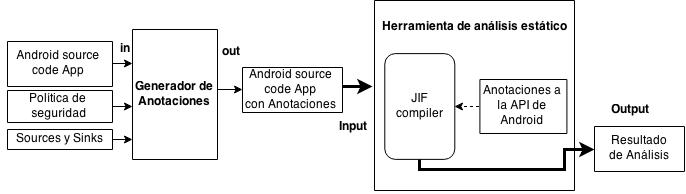
\includegraphics[width=9cm]{desing3Real-2-2.jpg} 
		\end{center}
	\end{figure}
\end{frame}
\begin{frame}{Política de Seguridad}
	\begin{columns}[c]
	\column{1.5in}
	\begin{center}
	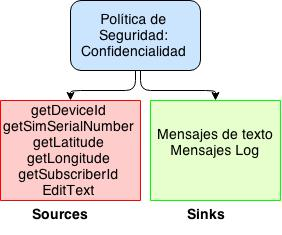
\includegraphics[width=5cm]{Politica.jpg} 
	\end{center}
	\column{1.5in}
	Flujos de información entre: información con nivel de seguridad alto e
	información con nivel de seguridad bajo.
	\end{columns}
\end{frame}

\subsection{Lineamientos de Anotación} 
\begin{frame}{Autoridad y Labels de Anotación}
	\center{Autoridad Máxima}
	\begin{center}
	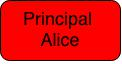
\includegraphics[width=3cm]{Principal.jpg}
	\end{center}
	\begin{columns}[c]
	\column{1.5in}
	\begin{center}
	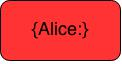
\includegraphics[width=3cm]{high.jpg}
	\end{center}
	Nivel de Seguridad Alto
	\column{1.5in}
	\begin{center} 
	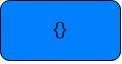
\includegraphics[width=3cm]{low.jpg}
	\end{center}
	Nivel de Seguridad Bajo\newline
	\end{columns}
\end{frame}	
\begin{frame}{Anotaciones a la API} %Anotaciones para
	\begin{block}{Controlar canales} 
	\begin{itemize}
	  \item Mensajes de texto (SmSManager)
	  \item Mensajes log (Log)
	\end{itemize} 
	\end{block}
	\begin{block}{Clases adicionales requeridas}
		\begin{itemize}
		  \item Clases para los sources
		  \item Clases para métodos de sobresscritura
		\end{itemize}
	\end{block}
\end{frame}	
\begin{frame}[fragile]{Controlar canales}
\begin{lstlisting}
sendTextMessage{Alice:}(String{Alice:}destAdd, 
		String{Alice:}scAdd, 
		String{} text,
	    PendingIntent{Alice:} sentIntent,
		PendingIntent{Alice:} deliveryIntent) { }
\end{lstlisting}
\end{frame}
\begin{frame}{Clases adicionales requeridas}
	\begin{block}{Mecanismos}
		\begin{itemize}
		  \item Anotación
		  \item Signaturas Nativas
		  \item signaturas nativas más labels de Seguridad
		\end{itemize}
	\end{block}
\end{frame}

\begin{frame}{Anotaciones para Integrar Clases de la API}
	\begin{figure}[t!]
		\begin{center} 
		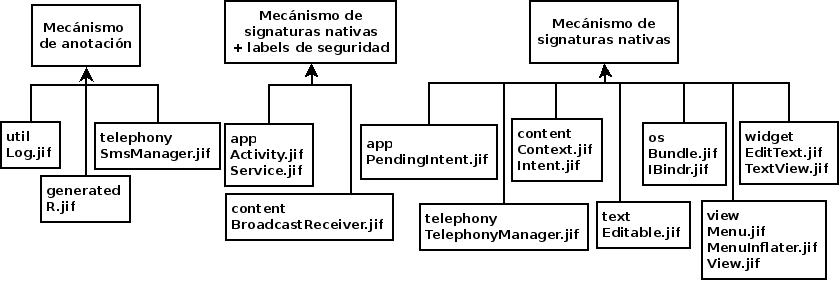
\includegraphics[width=9cm]{annotationsMechanims.jpeg} 
		\end{center}
	\end{figure}
\end{frame}

\begin{frame}
	\begin{center}
		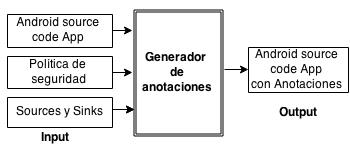
\includegraphics[width=4cm]{desingSolution2-2.jpg}
	\end{center}
\end{frame}

\begin{frame}{Anotación de aplicativos a analizar}{Generador de anotaciones}
\begin{block}{Objetivo de la anotación}
	\begin{itemize}
	  \item Métodos source contenidos en la clase
	  \item Métodos que influencian el source
	  \item Envio de información hacia canales con nivel de seguridad bajo
	\end{itemize}
\end{block}	
\pause	
\begin{block}{Lo que se anota}
	\begin{itemize}
	  \item Variables source
	  \item Métodos source
	  \item Método no source
	\end{itemize}
\end{block}		
\end{frame}




